%!TEX root = ../../PhD_thesis__Edouard_Leurent.tex

\graphicspath{{2-Chapters/1-Chapter/}}

\chapter{Introduction}
\label{chapter:1}

\begin{flushright}
	\begin{tabular}{@{}l@{}}
		\emph{Pour soulever un poids si lourd,}\\
		\emph{Sisyphe, il faudrait ton courage !}\\
		\emph{Bien qu’on ait du cœur à l’ouvrage,}\\
		\emph{L’Art est long et le Temps est court.}\\
	\end{tabular}

	Charles Baudelaire, \href{https://eleurent.github.io/sisyphe/texts/le-guignon.html}{\emph{Le guignon}}.
\end{flushright}

\section{Context and scope}


\subsection{How should a driving robot make decisions?}

In the first few weeks of my PhD, I observed that layman interlocutors, when confronted to this question on the occasion of a social dinner, have a general tendency to conjure up disaster scenarios involving imminent accidents with unavoidable casualties. This reflex is likely to stem from the popularisation of the Trolley Problem \citep{Foot1967}, a famous thought experiment in Moral Philosophy, depicted in \Cref{fig:trolley}, in which a runaway trolley is headed straight toward five people tied up on the main track and unable to move. A lever, when pulled, switches the trolley to a side track occupied by one person: what should you do? Answering this general question of what we \emph{ought} to do in any situation, what is a \emph{right} or \emph{wrong} decision, is the focus of the field of {normative ethics}. This dilemma illustrates a clash between two schools of thought: utilitarianism and deontological ethics. According to utilitarians, the rightfulness of an action should be evaluated based on its consequences, and actions maximising a \emph{utility} --the happiness and well-being for the affected individuals-- should be preferred. Conversely, deontologists evaluate the morality of actions \emph{per se}, according to a series of rules, rather than based on their consequences. Although this problem was initially introduced as a thought experiment, its transposition to the context of autonomous driving and arguably more realistic scenarios made it heavily cited in discussions regarding safety \citep[e.g.][]{Lin2015,Bonnefon2016,Gogoll2017}. In early 2017, MIT’s Media Lab launched the \emph{Moral Machine} platform \citep{Awad2018}, in which members of the public were invited to select the morally acceptable decision out of several options available to an autonomous vehicle. The authors argued that the recovered global preference would provide \emph{"essential topics to be considered by policymakers"}, and \citep{Noothigattu2018} proposed an implementation of a system aggregating these preferences, trained on the collected data. However, the relevance of this analogy to inform engineering and policy has been called into question. Thus, \citep{DeFreitas2019} point out that such dilemma are unlikely to occur on real roads, hard to detect by perception systems and to act upon by control systems, and that they are distracting researchers from the more appropriate goal of how to avoid accidents altogether. Indeed, when we drive we seldom find ourselves in such extreme situations but rather constantly ponder over less tragic questions-- where does this vehicle intend to go? do I have the time to proceed? what is the appropriate speed to drive at right now? Thus, artificially reproducing this cognitive process of driving while avoiding accidents is more of a technical problem than an ethical one, and will constitute the object of this thesis. Yet, it would be illusory to pretend that the practical implications of the Trolley Problem cannot simply be swept aside and replaced by technicality: we will see that ethical concerns still underpin most assumptions and design choices of safety-critical software.

\begin{figure}[tp]
	\centering
	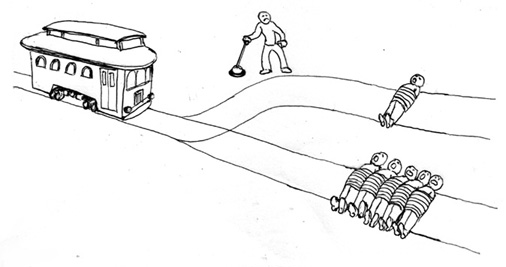
\includegraphics[width=0.7\linewidth]{img/trolley}
	\caption{The Trolley Problem \citep{Foot1967}. Illustration by \href{http://subcortex.com/}{Jesse J. Prinz}.}
	\label{fig:trolley}
\end{figure}

\subsection{Nuts and bolts of self-driving software}

\begin{figure}[th]
	\centering
	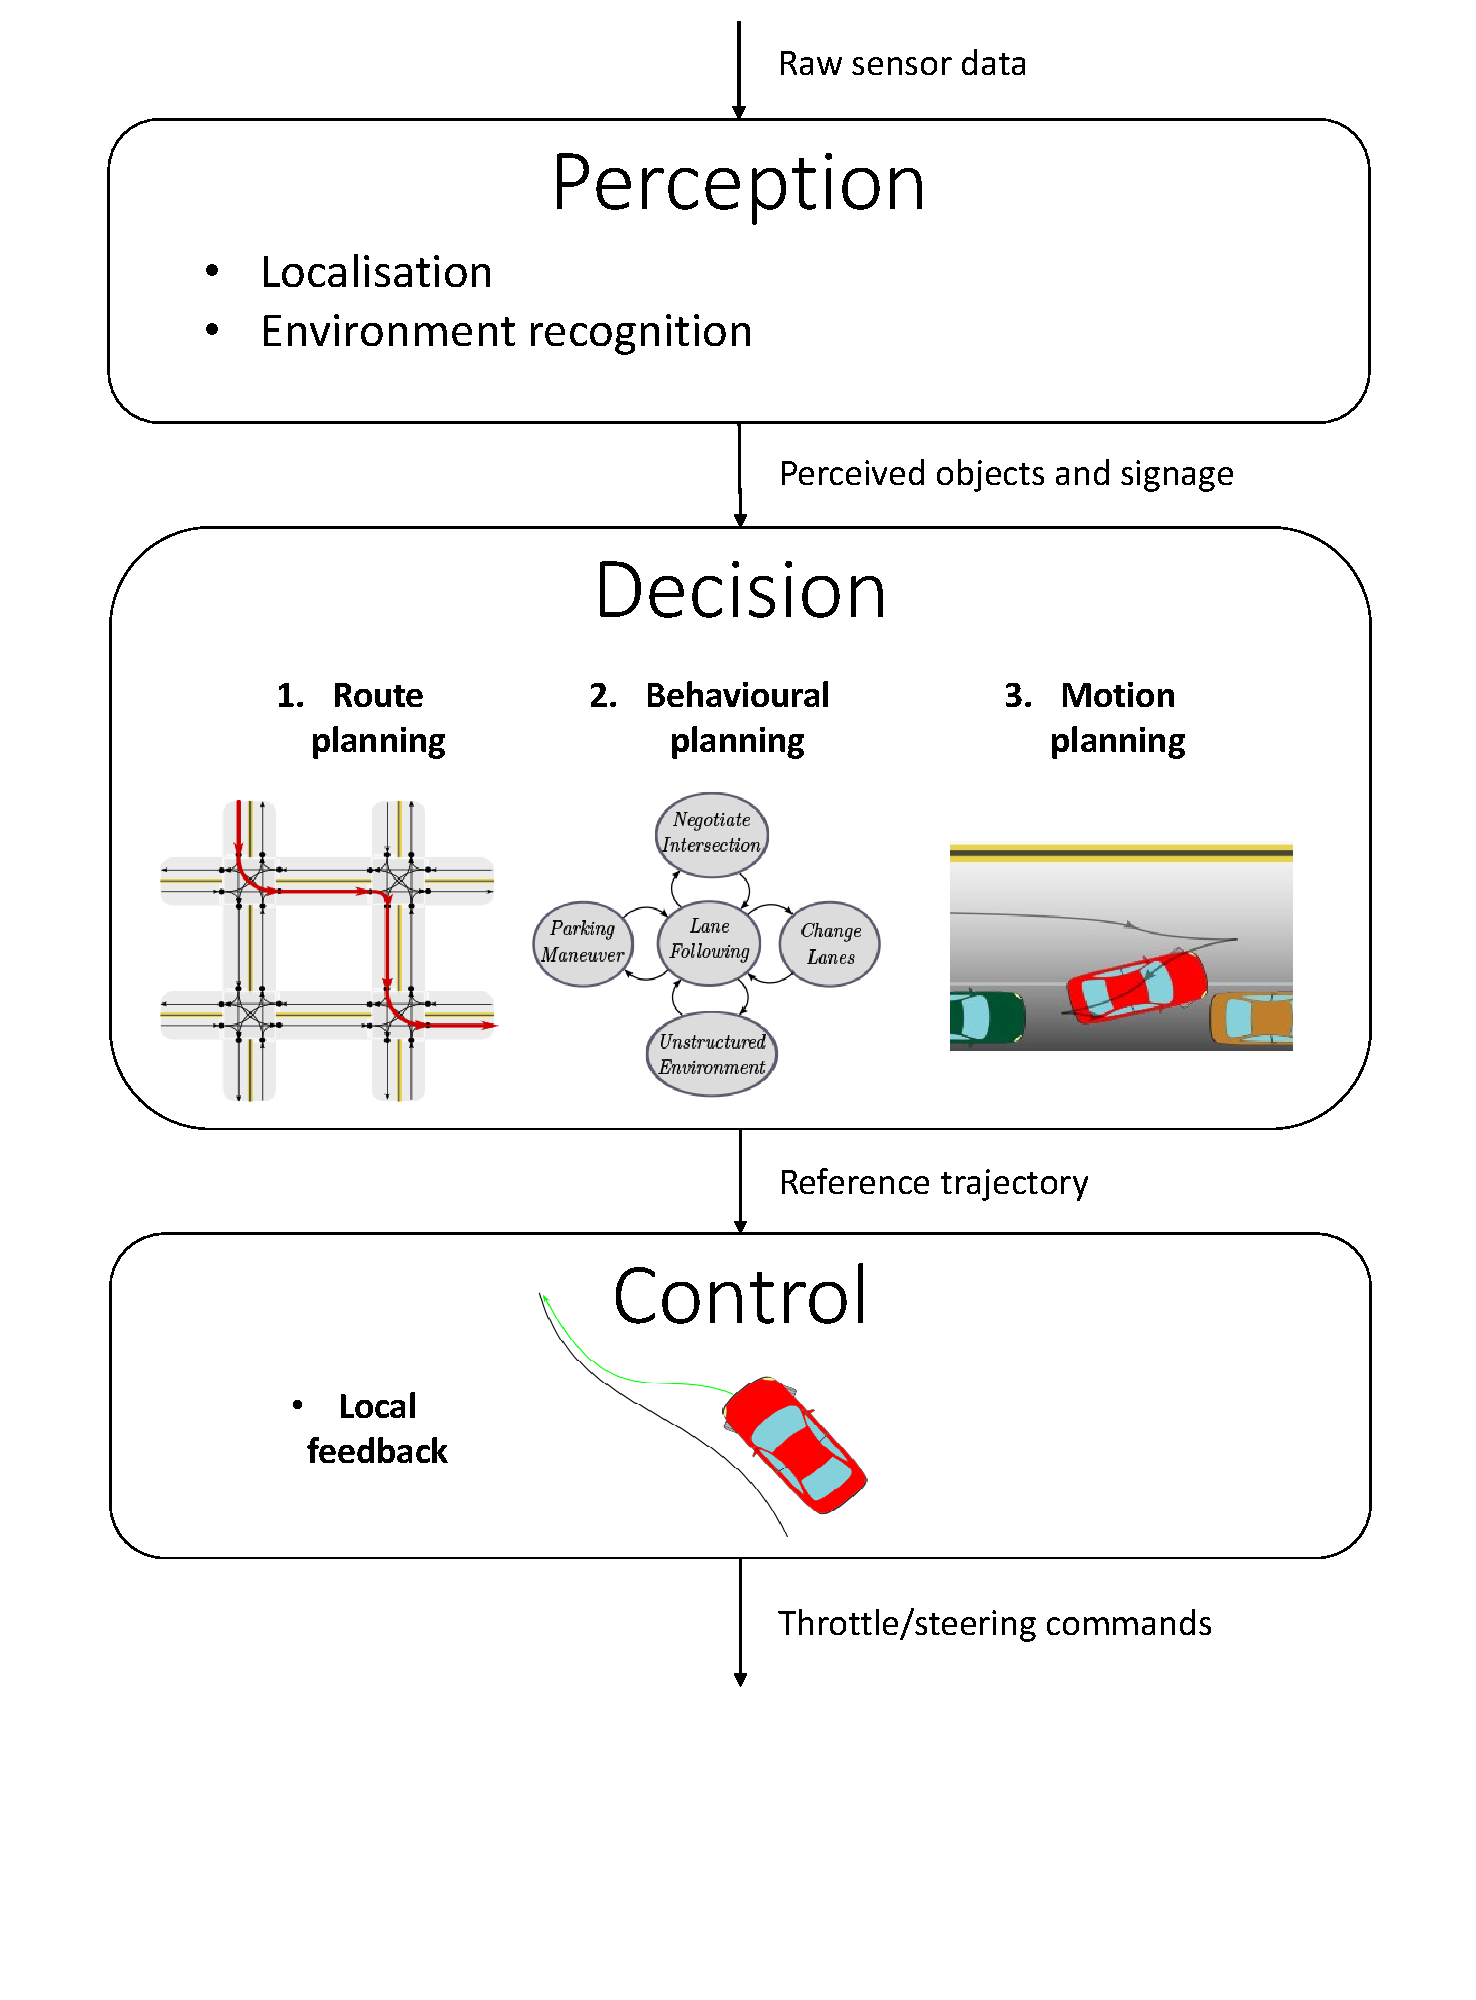
\includegraphics[trim={0 5cm 0 0}, clip, width=0.7\linewidth]{img/pipeline}
	\caption{The architecture of a typical self-driving software}
	\label{fig:robotics-pipeline}
\end{figure}

The traditional robotics pipeline, shown in \Cref{fig:robotics-pipeline}, involves three main tasks: \emph{Perception}, \emph{Decision}, and \emph{Control} (also called the Sense-Plan-Act paradigm, or Navigation, Guidance and Control in aerospace engineering). The \emph{Perception} module takes raw sensor data as input and produces a high-level reconstruction of the scene. The \emph{Decision} module then determines the desired trajectory of the vehicle, based on the current situation. Finally, the \emph{Control} module manipulates forces, by way of steering and throttle controls, to track the desired trajectory. In the context of Autonomous Driving, the Decision module is often implemented with a hierachical structure whose layers work at different timescales. First, a \emph{Route Planning} module searches for the shortest route in a road network from the current location to the desires destination. Second, the \emph{Behavioural Layer} specifies a coarse driving behaviour through short-term goals or semantic decisions, such as choosing to change lane, to slow down at an intersection, or to yield to a vehicle. This layer is thus responsible for following the planned route while adapting to the current traffic state in real time. Third, the \emph{Motion Planning} layer generates a continuous, feasible trajectory that implements the desired behaviour, while ensuring comfort and safety.

Great strides have been made in the two end-of-pipe tasks: Perception has benefited from the substantial progress in the field of Computer Vision due to the recent advent of Deep Learning, and many control schemes \citep[surveyed in][]{Polack2018} have been developed for ground vehicles. Even in the Decision module, Route Planning is virtually solved and already provided by services such as \href{https://wiki.openstreetmap.org/wiki/Routing}{Open Street Maps}, and there exist a vast body of Motion Planning algorithms, presented in \Cref{sec:sequential-decision-making}. All these building blocks are widely used in both industrial applications, including ADAS functions such as LKA, ACC, or AES, and in academic reasearch challenges. Ultimately, we claim that Behavioural Planning remains the only neglected link in the chain. Indeed, most of these applications focused hitherto on simple settings with little complexity: ADAS systems are mostly tailored for highway driving and struggle when merges and interaction. [ref needed]. Similarly, most academic challenges focused on highway driving, with the exception of the DARPA Urban challenge which required more advanced interactions with other vehicles. Yet, even this event still consituted a controlled environment, simple enough that all participants merely relied on rule-based systems for behavioural planning \citep{Buehler2009}, such as finite state machines whose transitions are triggered by handcrafted criteria \citep[\eg][]{Baker2008}. Yet, there is little hope that this approach can scale to complex scenes, and unit responses cannot be easily merged.

\subsection{Scope and Challenges of this Thesis}

\paragraph{Challenge 1: Decision-making under uncertainty: humans in the loop}
Even if we had magically access to magical perception and control, would we have solved the problem? What remains to do?
Why is it difficult?

- humans in the loop, with uncertain behaviours

Even if the present is known, the future is still uncertain.
We do not know how to model a human driver.
Human driving behaviour is not deterministic, but it is predictable. Highly structured.

Idea -> leverage data and sequential learning, to hope for better exhausivity.
We want to quantify uncertainty
Recall aletoric vs epistemic uncertainty?

\paragraph{Challenge 2: Social interactions and coupled dynamics}
- complex dynamics: coupling -> fast propagation of uncertainty, not isolated.
We want socially aware decision-making (account for other agents, and how our actions impact their behaviours)
We want to contain the uncertainty build up, prevent instability.

\paragraph{Challenge 3: Safety and efficiency}
- multiple contradictory objectives, interplay, hard to specify: defensive / aggressive tradeoff and negotiation.
the pitfall of reward engineering.
- how to guarantee safety for a leaning system, in the presence of uncertainty?
We want to formalize a notion of risk. Risk as a constraint ? As a worst-case outcome?

\section{Contributions}

Two approaches to sequential learning: model-free and model-based.

\paragraph{List of publications}